\chapter{Linear Algebra}

\section{Fundamental Building Blocks}%
\label{subsec:label}

We will introduce some important subjects to know about deep learning from linear algebra.

A \textbf{scalar} is simply a number. Usually \(x \in \mathbb{R}\) or \(x \in \mathbb{N}\).

A \textbf{vector} is an array of numbers, arranged in order. You can identify each number in the vector by an index.
\begin{equation*}
	\mathbf{x} = \begin{bmatrix} x_1 \\ \vdots \\ x_d \end{bmatrix}
	\quad \text{and} \quad
	\mathbf{x}^T = [x_1, \dots, x_d], \quad \mathbf{x} \in \mathbb{R}^d
\end{equation*}

By $\mathbb{R}^{d}$ it is meant that there are $d$ numbers, all of which real.
We think of vectors as points in space. Each element gives a coordinate along an axis.

A \textbf{matrix} is a 2D array of numbers. Like a vector, this is also identified by indices. However, for matrices there are two, as it has two dimensions.
\begin{equation*}
	\mathbf{A} = \begin{bmatrix} A_{1,1} & A_{1,2} \\ A_{2,1} & A_{2,2} \end{bmatrix}
\end{equation*}
You can also specify entire rows and columns: $A_{i:}$ is the $i$th row, and $A_{:j}$ is the $j$th column. Given a matrix with $m$ rows and $n$ columns called $A$, we say that $A \in \mathbb{R}^{m \times n}$.

A \textbf{tensor} is for when we need an array with more than two axes. An element $(i,j,k)$ of a tensor is denoted by $A_{i,j,k}$. \textbf{An example} of this is an RGB image: This is a tensor of height, width and colour channel. The number of axes is also denoted as \textbf{the rank} of the tensor.

\section{Vectors}%
\label{sec:vectors}

Vectors are often depicted as arrows in Euclidean space. Let us assume we have two vectors, $\mathbf{a}$ and $\mathbf{b}$.
\[
	\mathbf{a} = \begin{pmatrix} 1 \\ 3 \end{pmatrix}
	\quad \text{and} \quad
	\mathbf{b} = \begin{pmatrix} 4 \\ 2 \end{pmatrix}
\]

We can write those vectors as arrows. Seen in Figure~\ref{fig:aandb}, where $\mathbf{a}$ is the red arrow, and $\mathbf{b}$ is blue.
\begin{figure}[ht]
	\centering
	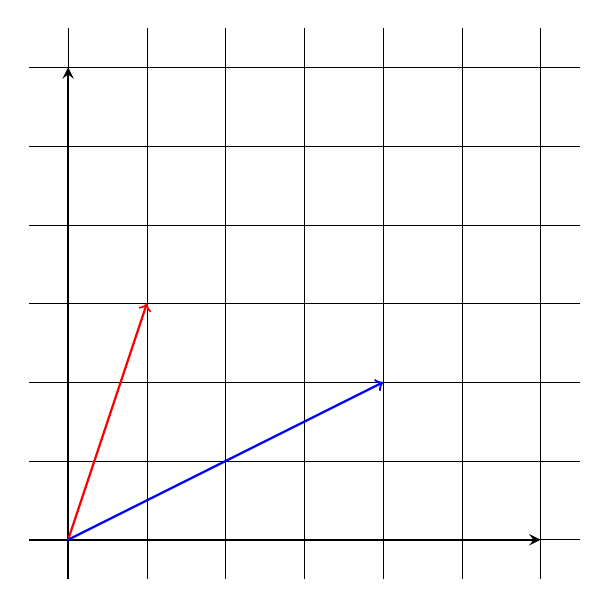
\begin{tikzpicture}
		% Draw axes
		\draw[thick, ->, >=stealth] (-0.5,0) -- (6,0) node[right] {};
		\draw[thick, ->, >=stealth] (0,-0.5) -- (0,6) node[above] {};

		% Draw grid
		\draw[very thin, black] (-0.5,-0.5) grid (6.5,6.5);

		% Draw vectors
		\draw[thick, ->, red] (0,0) -- (1,3);
		\draw[thick, ->, blue] (0,0) -- (4,2);
	\end{tikzpicture}
	\caption{\label{fig:aandb} $\mathbf{a}$ and $\mathbf{b}$}
\end{figure}

We can multiply vectors by a scalar. If we think of it Euclidean, the arrow will \textit{grow} by the size of the scalar. For example:

\[
	\mathbf{a} \cdot 2 = 2 \cdot \begin{pmatrix}
		1 \\
		3
	\end{pmatrix} = \begin{pmatrix}
		2 \cdot 1 \\
		2 \cdot 3
	\end{pmatrix} = \begin{pmatrix}
		2 \\
		6
	\end{pmatrix}
\]

The result can be found in Figure~\ref{fig:scalarmultiplicationtovectors}.
\begin{figure}[ht]
	\centering
	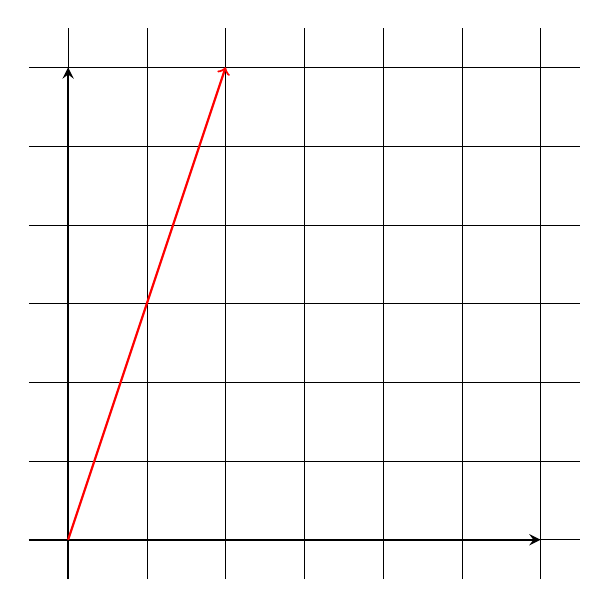
\begin{tikzpicture}
		% Draw axes
		\draw[thick, ->, >=stealth] (-0.5,0) -- (6,0) node[right] {};
		\draw[thick, ->, >=stealth] (0,-0.5) -- (0,6) node[above] {};

		% Draw grid
		\draw[very thin, black] (-0.5,-0.5) grid (6.5,6.5);

		% Draw vectors
		\draw[thick, ->, red] (0,0) -- (2,6);
	\end{tikzpicture}
	\caption{\label{fig:scalarmultiplicationtovectors} $\mathbf{a} \cdot 2$}
\end{figure}

You can also add two vectors together.
\[
	x+ y =
	\begin{pmatrix}
		x_{1}  \\
		\vdots \\
		x_{d}
	\end{pmatrix} + \begin{pmatrix}
		y_{1}  \\
		\vdots \\
		p_{d}
	\end{pmatrix} =
	\begin{pmatrix}
		x_{1} + y_{1} \\
		\vdots        \\
		x_{d} + y_{d}
	\end{pmatrix}
\]

The same goes for subtraction:

\[
	x+ y =
	\begin{pmatrix}
		x_{1}  \\
		\vdots \\
		x_{d}
	\end{pmatrix} - \begin{pmatrix}
		y_{1}  \\
		\vdots \\
		p_{d}
	\end{pmatrix} =
	\begin{pmatrix}
		x_{1} - y_{1} \\
		\vdots        \\
		x_{d} - y_{d}
	\end{pmatrix}
\]

When thinking of these Euclidian, you can think of one vector arrow being added or subtracted from the other, at the tip, such that ones beginning starts at the other's tip.

Another operation is the \textbf{dot product}. This gives us the result of a real number, rather than a vector as was the case before:

\[
	x \cdot y =
	\begin{pmatrix}
		x_{1}  \\
		\vdots \\
		x_{d}
	\end{pmatrix} \cdot \begin{pmatrix}
		y_{1}  \\
		\vdots \\
		p_{d}
	\end{pmatrix} =
	x_{1}y_{1} + x_{2}y_{2} + \cdots + x_{d}y_{d} = \sum_{i=1}^d x_{i}d_{i} = x^{T}y
\]

As the result is a scalar value, this is also called the scalar product or inner product. The dot product obeys many laws that hold for ordinary products of real numbers. Let $a,b,c$ be vectors and \(\lambda\) a scalar. Then:

\begin{enumerate}
	\item $a \cdot b = b \cdot a$
	\item $a \cdot (b + c) = a \cdot b + a \cdot c$
	\item $(\lambda a) \cdot b = \lambda(a \cdot b) = a \cdot (\lambda b)$
	\item \(0 \cdot a = 0\)
\end{enumerate}

The \textbf{length} of the vector is usually calculated as the square root of the summed squares of the entries:

\begin{equation*}
	|x| = \left| \begin{pmatrix}
		x_{1}  \\
		\vdots \\
		x_{d}
	\end{pmatrix} \right|
	=
	\sqrt{x_{1}^{2}+ \cdots + x^{2}_{d}} = \left(  \sum_{i=1}^d x^{2}_{1} \right)^{\frac{1}{2}}
\end{equation*}

This is just a member of a family of \textit{norms}, called $L^{p}$ norms:

\begin{equation*}
	L^{p} = \left(  \sum_{i} |x_{i}|^{p} \right)^{\frac{1}{p}}
\end{equation*}

$L^{2}$ norm is the most commonly used, and if nothing else is stated, this is the norm used. Also called the Euclidian norm. The max norm is $L^{\infty} = \left| \left| x \right| \right|_{\infty} = \max \left| x_{i} \right|$.

The dot product of two vectors can be written in terms of their $L^{2}$ norms and an angle \(\theta\) between them:

\[
	x \cdot y = |x| |y| \cdot \cos \theta
\]

Example with the previous two vectors we used, $\mathbf{a}$ and $\mathbf{b}$:
\[
	\theta = \cos^{-1} \left( \frac{\mathbf{a}\mathbf{b}}{|a| \cdot |b|} \right)
\]
\[
	= \cos^{-1} \left( \frac{10}{\sqrt{10} \cdot \sqrt{20}} \right) = 45^{\circ}
\]

\subsection{Matrices}%
\label{subsec:matrices}

The \textbf{order} of the matrix represents the number of rows and number of columns. For a matrix with 3 columns and 3 rows, the order would be $3 \times 3$. This is an example of a \textbf{square matrix}, which is a matrix whose column and row size is equal. There are also a few special matrices:
\begin{itemize}
	\item \textit{Row Matrix}: If a matrix only has one row: also a transposed vector
	\item \textit{Column Matrix}: If a matrix only has one column: a vector
	\item \textit{$1 \times 1$ Matrix}: A Scalar
\end{itemize}

You add two matrices by adding each of their elements:
\[
	\begin{pmatrix} a & b \\ c & d \end{pmatrix}
	+ \begin{pmatrix} e & f \\ g & h \end{pmatrix}
	= \begin{pmatrix} a + e & b + f \\ c + g & d + h \end{pmatrix}
\]
It is necessary for the matrices to have the same order (or dimensionality).

You can also multiply a matrix by a scalar \(\lambda\):
\[
	\lambda \cdot \begin{pmatrix} a & b \\ c & d \end{pmatrix}
	= \begin{pmatrix} \lambda \cdot a & \lambda \cdot b \\ \lambda \cdot c & \lambda \cdot d \end{pmatrix}
\]

You can also multiply two matrices. To do this, you perform the dot product between rows of the first matrix and columns of the second matrix:
\[
	\mathbf{A \cdot B = C}
\]
\[
	c_{i,j} = \sum_k a_{ik}b_{kj}
\]

Thus two matrices can only be multiplied if the number of columns in the first matrix is equal to the number of rows in the second matrix. I.e., if \textbf{A} is of order $m \times n$ and \textbf{B} is of order $r \times s$, then $A \cdot B$ is possible if $r = n$. The resulting matrix will be of order $m \times s$.

There are some properties to the matrix product:
\begin{itemize}
	\item Distributivity over addition: \(A(B+C) = AB+AC\)
	\item Associativity: \(A(BC) = (AB)C\)
	\item \textbf{Not commutative}.
	      \begin{itemize}
		      \item However, is between two vectors: $x^{T}y = y^{T}x$
	      \end{itemize}
	\item Transpose of a matrix product has a simple form: $(AB)^{T} = B^{T}A^{T}$
\end{itemize}

The norm of a matrix is analogous to $L^{2}$ form of a vector:
\[
	||A|| = \left( \sum_{i,j} A_{i,j}^{2} \right)^{\frac{1}{2}}
\]

\subsection{Square Matrices}%
\label{subsec:label}

There are some operations special to square matrices, which are not defined for arbitrary matrices.

An \textit{identity matrix} (or unit matrix) of size $d$ is a square matrix of order $d \times d$ where all the diagonal elements are '1' and all other elements are '0'. It is denoted by $I$:
\[
	I_1 = (1) \quad
	I_2 = \begin{pmatrix} 1 & 0 \\ 0 & 1 \end{pmatrix} \quad
	I_3 = \begin{pmatrix} 1 & 0 & 0 \\ 0 & 1 & 0 \\ 0 & 0 & 1 \end{pmatrix}
\]

For a square matrix $A$, we have an important property:
\[
	A \cdot I = I \cdot A = A
\]

The \textbf{inverse} of a matrix is defined as being the matrix whose product with the original matrix produces an identity matrix:

\[
	AA^{-1} = A^{-1}A = I
\]

However, not all square matrices have inverses. Those who do are called \textit{invertible} or are said to be \textit{nonsingular matrices}. A square matrix which does not have an inverse is called noninvertible or singular matrix. A square matrix is singular if and only if its determinant is 0.

We will now look at \textit{determinants}. The determinant of a square matrix $det(A)$ is a mapping to a scalar. It is equal to the product of all eigenvalues of the matrix. It measures how much multiplication by the matrix expands or contracts space.

\noindent
\textbf{For a 1x1 matrix:}
\[
	\det(a_{11}) = a_{11}
\]

\noindent
\textbf{For a 2x2 matrix:}
\[
	\begin{vmatrix}
		a_{11} & a_{12} \\
		a_{21} & a_{22}
	\end{vmatrix}
	= a_{11}a_{22} - a_{12}a_{21}
\]

\noindent
\textbf{For a 3x3 matrix:}
\[
	\begin{vmatrix}
		a_{11} & a_{12} & a_{13} \\
		a_{21} & a_{22} & a_{23} \\
		a_{31} & a_{32} & a_{33}
	\end{vmatrix}
	= a_{11}(a_{22}a_{33} - a_{23}a_{32}) - a_{12}(a_{21}a_{33} - a_{23}a_{31}) + a_{13}(a_{21}a_{32} - a_{22}a_{31})
\]

\subsection{Special vectors and matrices}%
\label{subsec:label}

A \textit{unit vector} is a vector with unit norm $||x||_{2}=1$.

A vector $x$ and vector $y$ are said to be orthogonal to each other if $x^{T}y=0$. Meaning vectors are at 90 degrees to each other.

An \textit{orthogonal matrix} is a square matrix whose columns and rows are orthogonal unit vectors $A^{-1} = A^{T}$

A \textit{diagonal matrix} is a matrix with mostly zeroes, except for the diagonal, which contains non-zero entries. $diag(\mathbf{v})$ is a square diagonal matrix with diagonal elements given by entries of vector $\mathbf{v}$. Multiplying $diag(v)$ by vector $x$ only needs to scale each element $x_{i}$ by $v_{i}$.

A \texttt{symmetric matrix} is a matrix which is equal to its transpose:
\[
	A = A^{T}
\]

\section{Matrices as Linear Transformation}%
\label{sec:label}

A matrix defines a \textit{linear transformation}. A matrix represents a set of rules that tells you how to move a vector in space. You can think of a matrix like a machine that takes in a vector, and outputs another vector after having done some operations on the vector. We say the transformation is ``linear'' as it preserves operations like addition and scaling. The reason we care for matrices as linear transformations, is because they help us perform complex operations on vectors efficiently by condensing multiple operations (scaling, rotating, reflecting, etc.) into a single mathematical object.

A matrix $\mathbf{A} \in \mathbb{R}^{n \times m}$ projects points from $\mathbb{R}^{n}$ to their image in $\mathbb{R}^{m}$. If you have a vector $\mathbf{x} \in \mathbb{R}^{n}$, and a matrix $\mathbf{A} \in \mathbb{R}^{n \times m}$, then the matrix-vector multiplication $\mathbf{Ax}$ results in a new vector $\mathbf{y} \in \mathbb{R}^{m}$.

\begin{example}[3D to 2D space using a matrix]
	Given a vector $\mathbf{x} \in \mathbb{R}^{3}$ (i.e., in 3D space), and a matrix $\mathbf{A} \in \mathbb{R}^{2 \times 3}$, then the result is a vector in 2d space. Thus the transformation ``projects'' the vector from its 3D position to some new position in the 2D plane.
\end{example}

We can use matrices for the hidden layers in a neural network. Each hidden layer transforms the input in same way. Thus, using matrices makes it more manageable and the data flow more systematic.

\begin{example}[Reflection on the $x$-axis]
	\begin{equation*}
		\mathbf{M}x = \begin{vmatrix}
			1 & 0  \\
			0 & -1
		\end{vmatrix} \cdot \begin{vmatrix}
			x \\
			y
		\end{vmatrix} = \begin{vmatrix}
			x \\
			-y
		\end{vmatrix}
	\end{equation*}

	Having an image projection, using this matrix would effectively ``flip'' the image upside-down.
\end{example}

\section{System of Linear Equations}%
\label{sec:systemoflinearequations}

A system of linear equations, also called a linear system, is a collection of two or more linear equations involving the same set of variables. For example, the three linear equations following:
\begin{align*}
	a_{11}x_{1}a_{12}x_{2}a_{13}x_{3} & = b_{1} \\
	a_{21}x_{1}a_{22}x_{2}a_{23}x_{3} & = b_{2} \\
	a_{31}x_{1}a_{32}x_{2}a_{33}x_{3} & = b_{3}
\end{align*}

Can be represented as a matrix as such:
\[
	\begin{pmatrix}
		a_{11} & a_{12} & a_{13} \\
		a_{21} & a_{22} & a_{23} \\
		a_{31} & a_{32} & a_{33}
	\end{pmatrix}
	\begin{pmatrix}
		x_1 \\
		x_2 \\
		x_3
	\end{pmatrix}
	=
	\begin{pmatrix}
		b_1 \\
		b_2 \\
		b_3
	\end{pmatrix}
\]

And thus it becomes $\mathbf{Ax} = \mathbf{b}$. We are often in a situation where we are given $\mathbf{A}$ and $\mathbf{b}$ and are looking for an $\mathbf{x}$ to satisfy our system of linear equations. Every linear system may only have one of three possible solutions:
\begin{enumerate}
	\item The system has a single unique solution.
	\item The system has infinitely many solutions.
	\item The system has 0 solutions.
\end{enumerate}

If looking at it geometrically, you can think of the variables $x$ and $y$ as linear equations which determine a line on the $xy$-plane. Then the solutions are either:
\begin{enumerate}
	\item An intersection of the lines, thus having one solution.
	\item The lines themselves intersect throughout, thus having infinitely many solutions.
	\item The lines don't intersect at all, having 0 solutions.
\end{enumerate}

We say that a linear system is \textbf{consistent} if it has at least one solution, and \textbf{inconsistent} if it has zero. A linear system is said to be \textbf{independent} if none of the equations can be written as a linear combination of others. For example $x+y=2$ and $2x+2y=4$ are not, as the first can be obtained through division by the second, or the other way around.

\section{Matrix Decomposition}%
\label{sec:label}

You can decompose a matrix into \textit{factors} in order to learn about it's properties, which is not discernible from their representation.
In deep learning or data analysis, decomposing matrices can help uncover hidden patterns (e.g., the directions in which data varies the most). Decomposition allows us to look beyond the numbers in the matrix and understand the underlying structure.

An \textbf{eigenvector} of a square matrix \textbf{A} is a non-zero vector $\mathbf{v}$, such that multiplication by $\mathbf{A}$ only changes the scale of \textbf{$v$}. The only thing that happens to an eigenvector when a matrix $\mathbf{A}$ is applied to it is that it gets scaled by a constant (the eigenvalue).

If $Av = \lambda v$, $v$ is an eigenvector, and $\lambda$ is the corresponding eigenvalue.

Consider the operation $Av = w$. We are particularly interested in the special case when $v$ is an eigenvector, which means that the result of applying $A$ to $v$ doesn't change its direction, only its magnitude. This can be rewritten using the eigenvalue equation $Av = \lambda v$, where \(\lambda\) is the \textit{eigenvalue}, that describes the scale by which the vector scales.


\subsection{Eigendecomposition}%
\label{subsec:label}

Suppose that matrix $A$ has $n$ linearly independent eigenvectors $\{v^{(1)}, \ldots, v^{(n)}\}$ with the eigenvalues $\{\lambda_{1}, \ldots, \lambda_{n}\}$. We can concatenate the eigenvectors to get the matrix $V$. Furthermore, we can concatenate the eigenvalues and get a vector $\lambda = [\lambda_{1}, \ldots, \lambda_{n}]$ which is normally presented in descending order. The \textit{eigendecomposition} of $A$ is given by $A = Vdiag(\lambda)V^{-1}$

When you decompose a matrix $A$ into its eigenvectors and eigenvalues, you get a clearer picture of how the matrix transforms space. You can think of it as breaking down $A$ into simple, independent transformations that occur along specific directions (eigenvectors).

The decomposition expresses the matrix as a product of: $V$, a matrix of eigenvectors that define the important directions, and $diag(\lambda)$, a diagonal matrix that scales these eigenvectors by the corresponding eigenvalues.
This is useful because diagonal matrices are easy to work with — multiplication, inversion, etc., all become simpler.

Every real symmetric matrix $A$ can be decomposed into real-valued eigenvectors and eigenvalues.

A matrix whose eigenvalues are:
\begin{itemize}
	\item All positive is called \textbf{positive definite}
	\item All positive or zero-valued is called \textbf{positive semidefinite}
	\item All negative is called \textbf{negative definite}
	\item All negative or zero-valued is called \textbf{negative semidefinite}.
\end{itemize}












%%% Local Variables:
%%% mode: latex
%%% TeX-engine: luatex
%%% TeX-command-extra-options: "-shell-escape"
%%% TeX-master: "main"
%%% End:
